\documentclass[11pt,a4paper]{article}

\usepackage[margin=25mm]{geometry}
\usepackage{graphicx}
\usepackage{booktabs}
\usepackage{amsmath}
\usepackage{hyperref}
\usepackage{caption}
\usepackage{subcaption}
\usepackage{xcolor}

\title{Monospecies Biofilm: TMCMC Parameter Estimation\\
with Dynamic Nutrient Coupling and Extended $a_{11}(T)$ Models}
\author{Keisuke Nishioka}
\date{\today}

\begin{document}
\maketitle

\tableofcontents
\bigskip

% ─────────────────────────────────────────────────────────────────────────────
\section{Introduction}
% ─────────────────────────────────────────────────────────────────────────────
Biofilm growth exhibits strong temperature dependence and nutrient-limited dynamics.
This report estimates the temperature-dependent growth-attachment rate $a_{11}$ of a
monospecies Hamiltonian ODE model using Transitional Markov Chain Monte Carlo (TMCMC),
and evaluates the impact of dynamic nutrient coupling
\[
  c(t) = c_{\mathrm{scale}} \left(1-\phi(t)\psi(t)\right).
\]
The temperature set and data follow \cite{liu2019}.

Three modelling expansions are addressed in order of increasing complexity:
\begin{enumerate}
  \item \textbf{Static-temperature} estimation: 1-parameter (M1, $a_{11}$),
        3-parameter (M3, add $c_{\mathrm{scale}}$ and $\phi_0$), and
        4-parameter (M4, additionally add attachment inertia $\eta_\phi$).
  \item \textbf{Dynamic-temperature (Dy)} validation with three static-to-dynamic
        transfer models: 1-var, 8-var (multi-knot), and Ratkowsky.
  \item \textbf{Enhanced $a_{11}(T,t)$ models}: CTM, thermal-memory,
        asymmetric-lag, and composite variants.
\end{enumerate}

% ─────────────────────────────────────────────────────────────────────────────
\section{Methodology}
% ─────────────────────────────────────────────────────────────────────────────
\subsection{Hamiltonian ODE}
The monospecies biofilm state vector is $(\phi,\,\psi,\,\phi_0)$, where $\phi$
is the bacterial volume fraction, $\psi$ is the elastic stretch ratio, and
$\phi_0=1-\phi$ is the EPS/void fraction. The governing ODEs are
\begin{align}
    \frac{d\phi}{dt} &= a_{11}(T,t)\cdot\phi\cdot\frac{c}{c+K_p}, \label{eq:phi}\\
    \frac{d\psi}{dt} &= -\eta_{\phi}\frac{d\phi}{dt}\cdot\psi
                        -\eta\,\psi\ln\psi, \label{eq:psi}
\end{align}
where $a_{11}(T,t)$ is the temperature- and time-dependent growth-attachment rate,
$c$ is the local nutrient concentration, $K_p$ is the Monod half-velocity constant,
and $\eta,\,\eta_\phi$ are elastic-relaxation and attachment-inertia coefficients.
The observable is $\bar\phi(t)=\phi(t)\psi(t)$ (biofilm history).

\subsection{Dynamic Nutrient Coupling}
\begin{equation}
    c(t) = c_{\mathrm{scale}}\cdot\max\!\bigl(1-\bar\phi(t),\,0\bigr).
\end{equation}
Two cases were tested in early experiments: $c_{\mathrm{scale}}\in\{10,100\}$.
All subsequent results use $c_{\mathrm{scale}}=10$ as default unless stated.

\subsection{Observation Mapping (Profiled Likelihood)}
At observation times, we map $\bar\phi$ to $\log_{10}(\mathrm{CFU/mL})$ via an
affine model $y \approx a\,\bar\phi+b$, where $(a,b)$ are solved analytically by
least squares for each parameter draw (profiled likelihood).

\subsection{Numerical Integration}
Implicit Euler with $N_{\mathrm{newton}}=6$ Newton iterations per time step;
$\Delta t=10^{-4}$, consistent between estimation and post-processing.

\subsection{TMCMC}
Transitional MCMC \cite{ching2007} with Random-Walk (RW) mutation; GPU-accelerated via
\texttt{jax.vmap} over $N_p$ particles. All runs use $N_p\ge 2000$ unless noted.

% ─────────────────────────────────────────────────────────────────────────────
\section{Static Temperature Results}
% ─────────────────────────────────────────────────────────────────────────────
\subsection{Model Hierarchy: M1 → M3 → M4}
Three parameter sets were estimated for each of the eight static temperatures
$T\in\{4,8,15,20,25,35,37,40\}$\,°C:

\begin{description}
  \item[M1] $\theta=(a_{11})$; $c_{\mathrm{scale}}=10$, $\phi_0=0.1$, $\eta_\phi=1$.
  \item[M3] $\theta=(a_{11},\,c_{\mathrm{scale}},\,\phi_0)$; $\eta_\phi=1$ fixed.
  \item[M4] $\theta=(a_{11},\,c_{\mathrm{scale}},\,\phi_0,\,\eta_\phi)$; all free.
\end{description}

\begin{table}[h]
\centering
\caption{RMSE comparison: M1→M3→M4 static estimation (MAP, profiled affine fit, all 8 temperatures).
         M1: $c(t)=10(1-\phi\psi)$, $\theta=(a_{11})$.
         M3: $\theta=(a_{11},c_{\rm scale},\phi_0)$.
         M4: $\theta=(a_{11},c_{\rm scale},\phi_0,\eta_\phi)$.}
\begin{tabular}{rccccc}
\toprule
$T$ (°C) & M1 RMSE & M3 RMSE & M4 RMSE & $\Delta$(M1→M3) & $\Delta$(M3→M4) \\
\midrule
 4  & 0.176 & 0.145 & 0.139 & $-$0.031 & $-$0.006 \\
 8  & 0.100 & 0.050 & 0.037 & $-$0.051 & $-$0.013 \\
15  & 0.149 & 0.085 & 0.086 & $-$0.063 & $+$0.001 \\
20  & 0.241 & 0.198 & 0.197 & $-$0.043 & $-$0.001 \\
25  & 0.144 & 0.078 & 0.080 & $-$0.067 & $+$0.002 \\
35  & 0.191 & 0.104 & 0.098 & $-$0.087 & $-$0.007 \\
37  & 0.294 & 0.185 & 0.152 & $-$0.108 & $-$0.034 \\
40  & 0.217 & 0.117 & 0.090 & $-$0.100 & $-$0.027 \\
\midrule
\textbf{Mean} & \textbf{0.189} & \textbf{0.120} & \textbf{0.110} & $-$0.069 & $-$0.011 \\
\bottomrule
\end{tabular}
\label{tab:rmse_comparison}
\end{table}

Key observations:
\begin{itemize}
  \item M1 already achieves good fits ($R^2 > 0.97$ for most temperatures) with only
        a single free parameter, demonstrating that $c(t)=10(1-\phi\psi)$ captures
        the growth dynamics well.
  \item Adding $c_{\mathrm{scale}}$ and $\phi_0$ (M1→M3) gives the largest RMSE reduction
        (mean $-$0.069; up to $-$0.108 at 37\,°C, $-53\%$ at 8\,°C).
  \item Adding $\eta_\phi$ (M3→M4) provides additional improvement primarily at
        high-growth temperatures (37\,°C: $-18\%$; 40\,°C: $-23\%$; 8\,°C: $-27\%$).
        At 15\,°C and 25\,°C $\eta_\phi$ saturates, suggesting it is only identifiable
        in fast-growth regimes.
\end{itemize}

\begin{figure}[h]
\centering
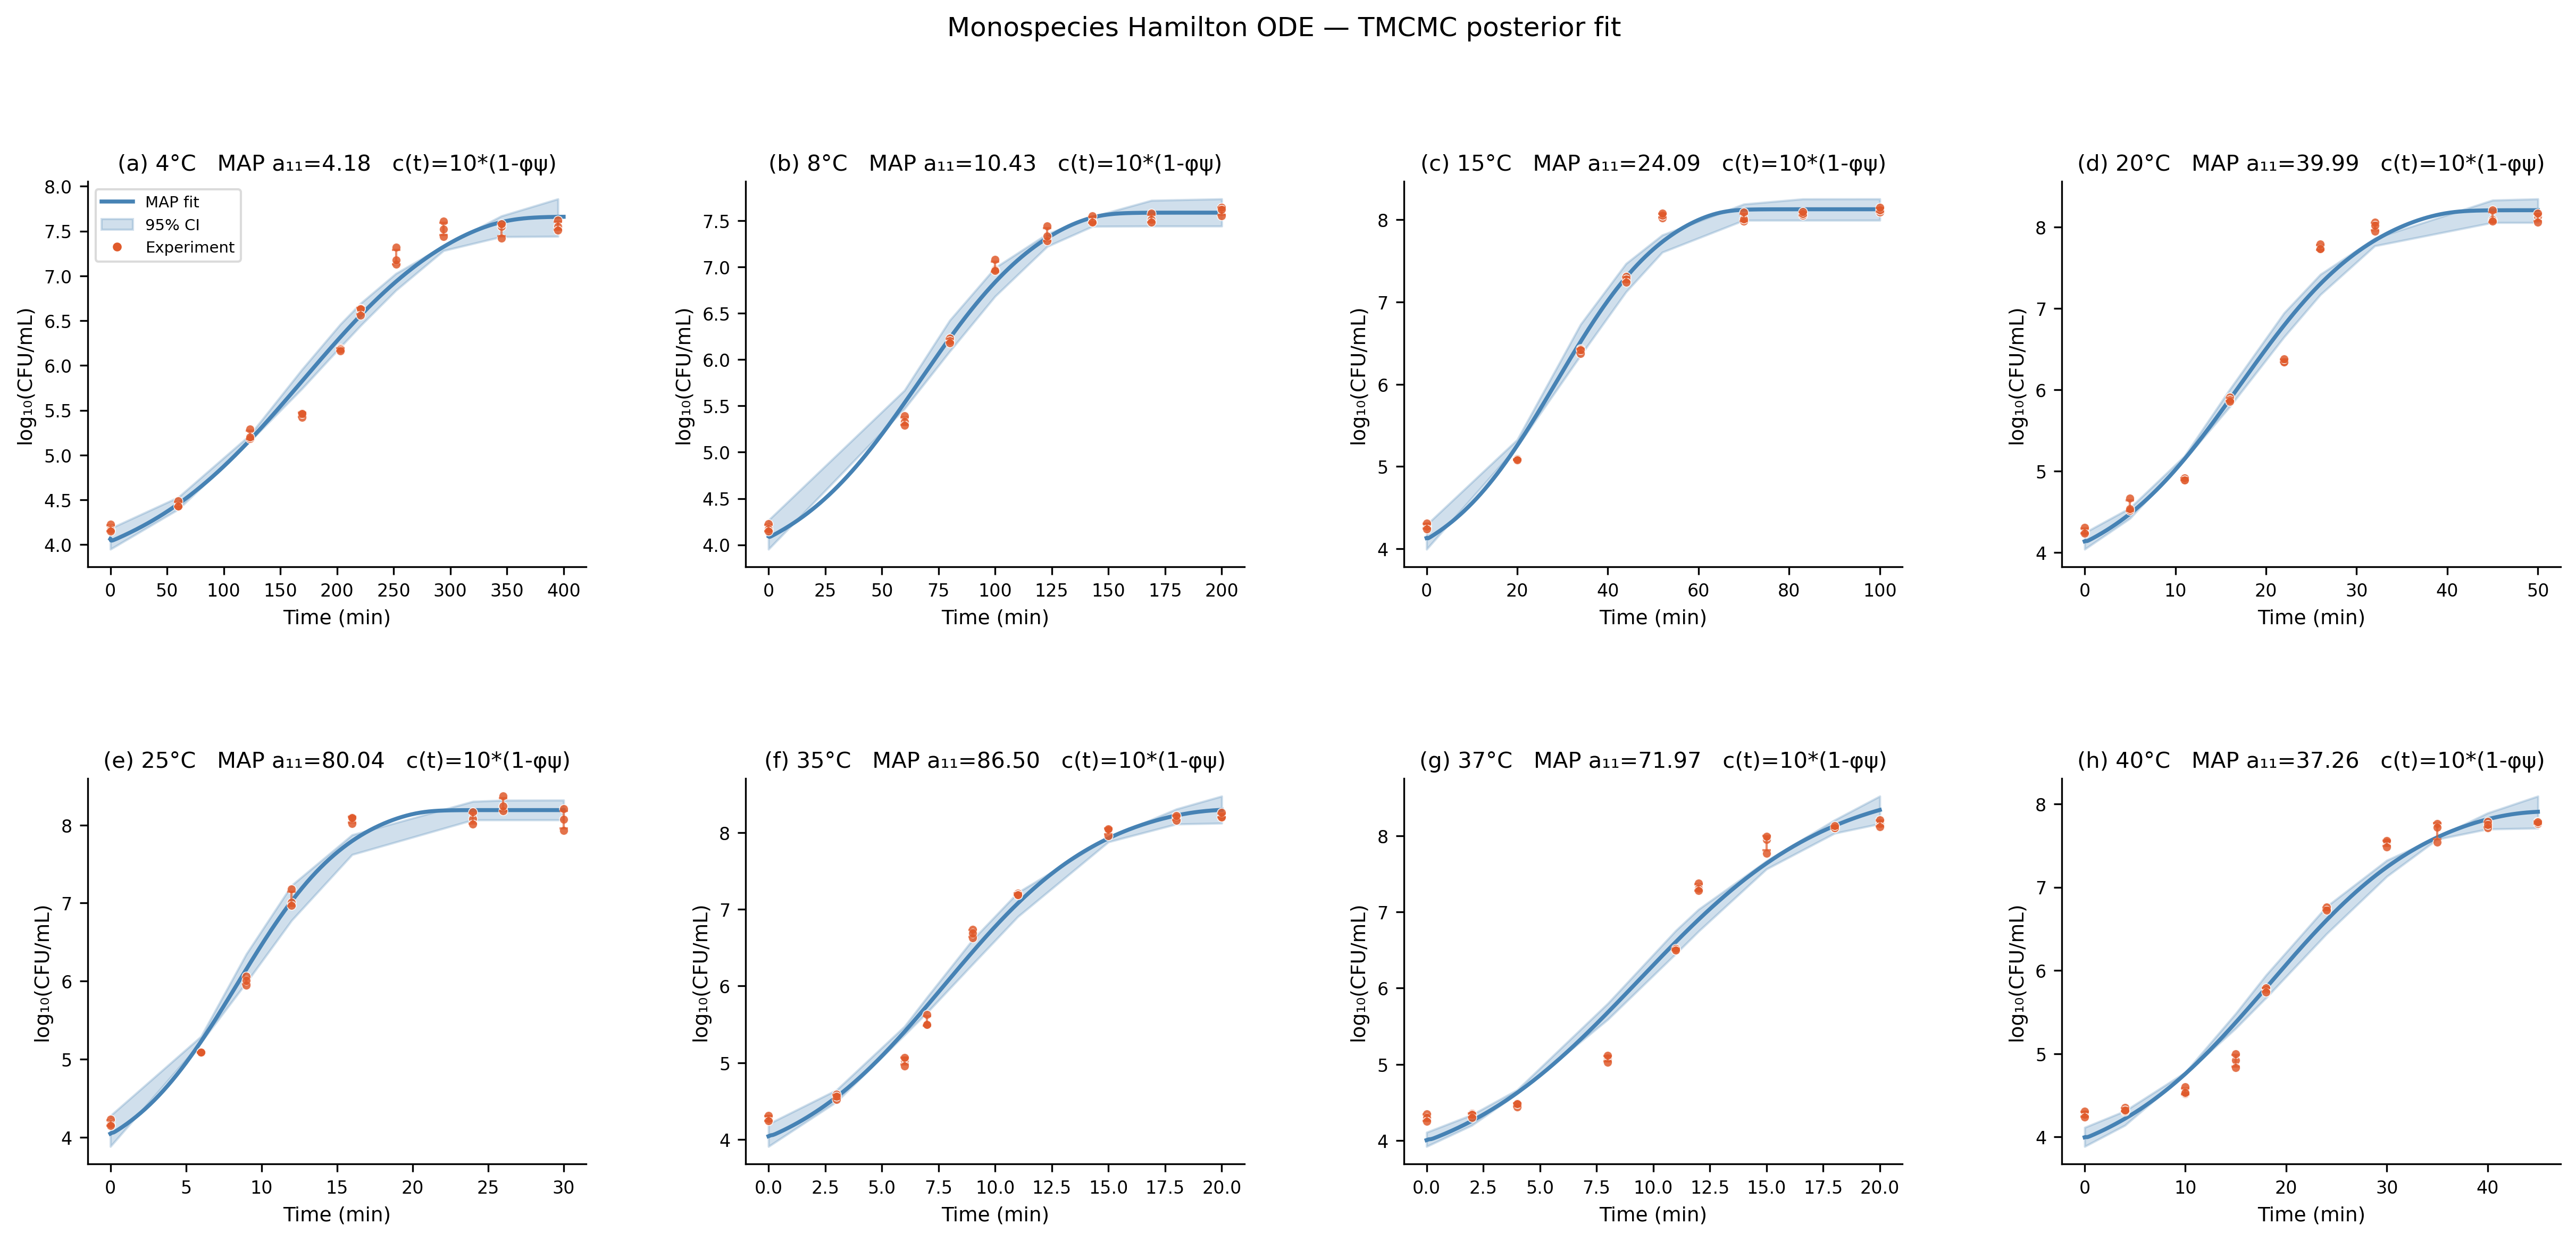
\includegraphics[width=\textwidth]{figures/monospecies_8panel_dyncc10_a11.png}
\caption{M1 TMCMC results ($\theta = a_{11}$ only, $c_{\mathrm{scale}}=10$ fixed) for all eight
         static temperatures. Blue: MAP trajectory; shaded band: 95\% posterior predictive CI;
         orange: experimental means.}
\label{fig:1d_8panel}
\end{figure}

\begin{figure}[h]
\centering
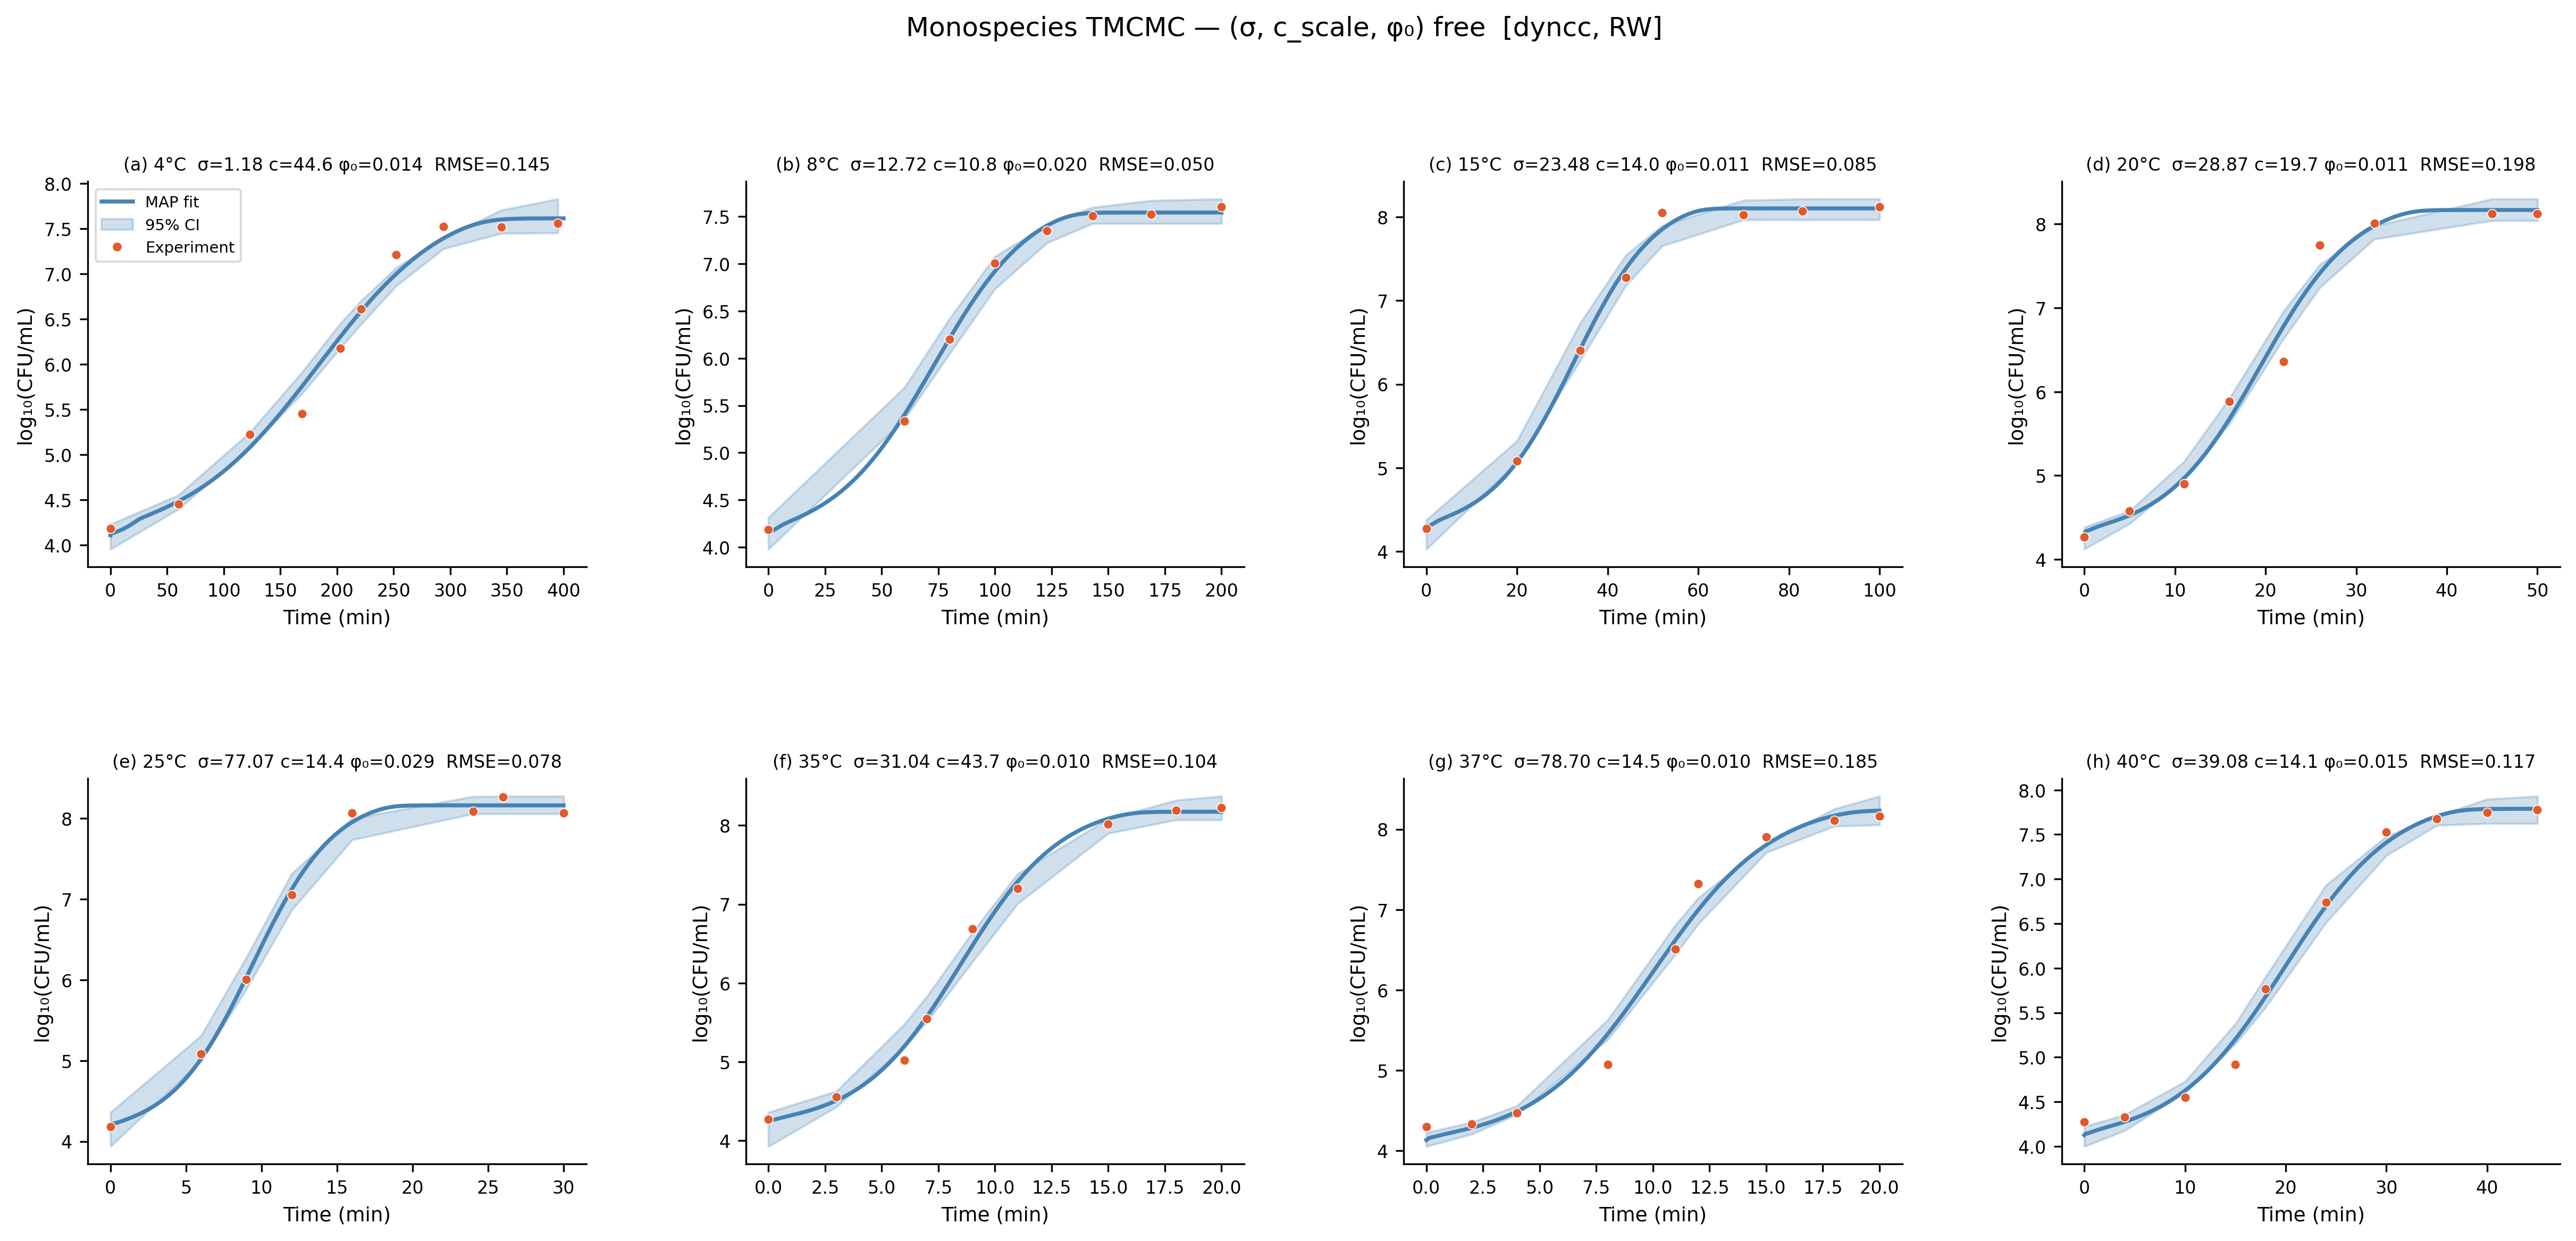
\includegraphics[width=\textwidth]{figures/monospecies_8panel_3param.png}
\caption{M3 TMCMC ($\theta = a_{11}, c_{\mathrm{scale}}, \phi_0$; MAP + 95\% posterior predictive CI)
         for all eight temperatures. Blue: MAP trajectory; shaded band: 95\% CI; orange: experimental means.}
\label{fig:3d_8panel}
\end{figure}

\begin{figure}[h]
\centering
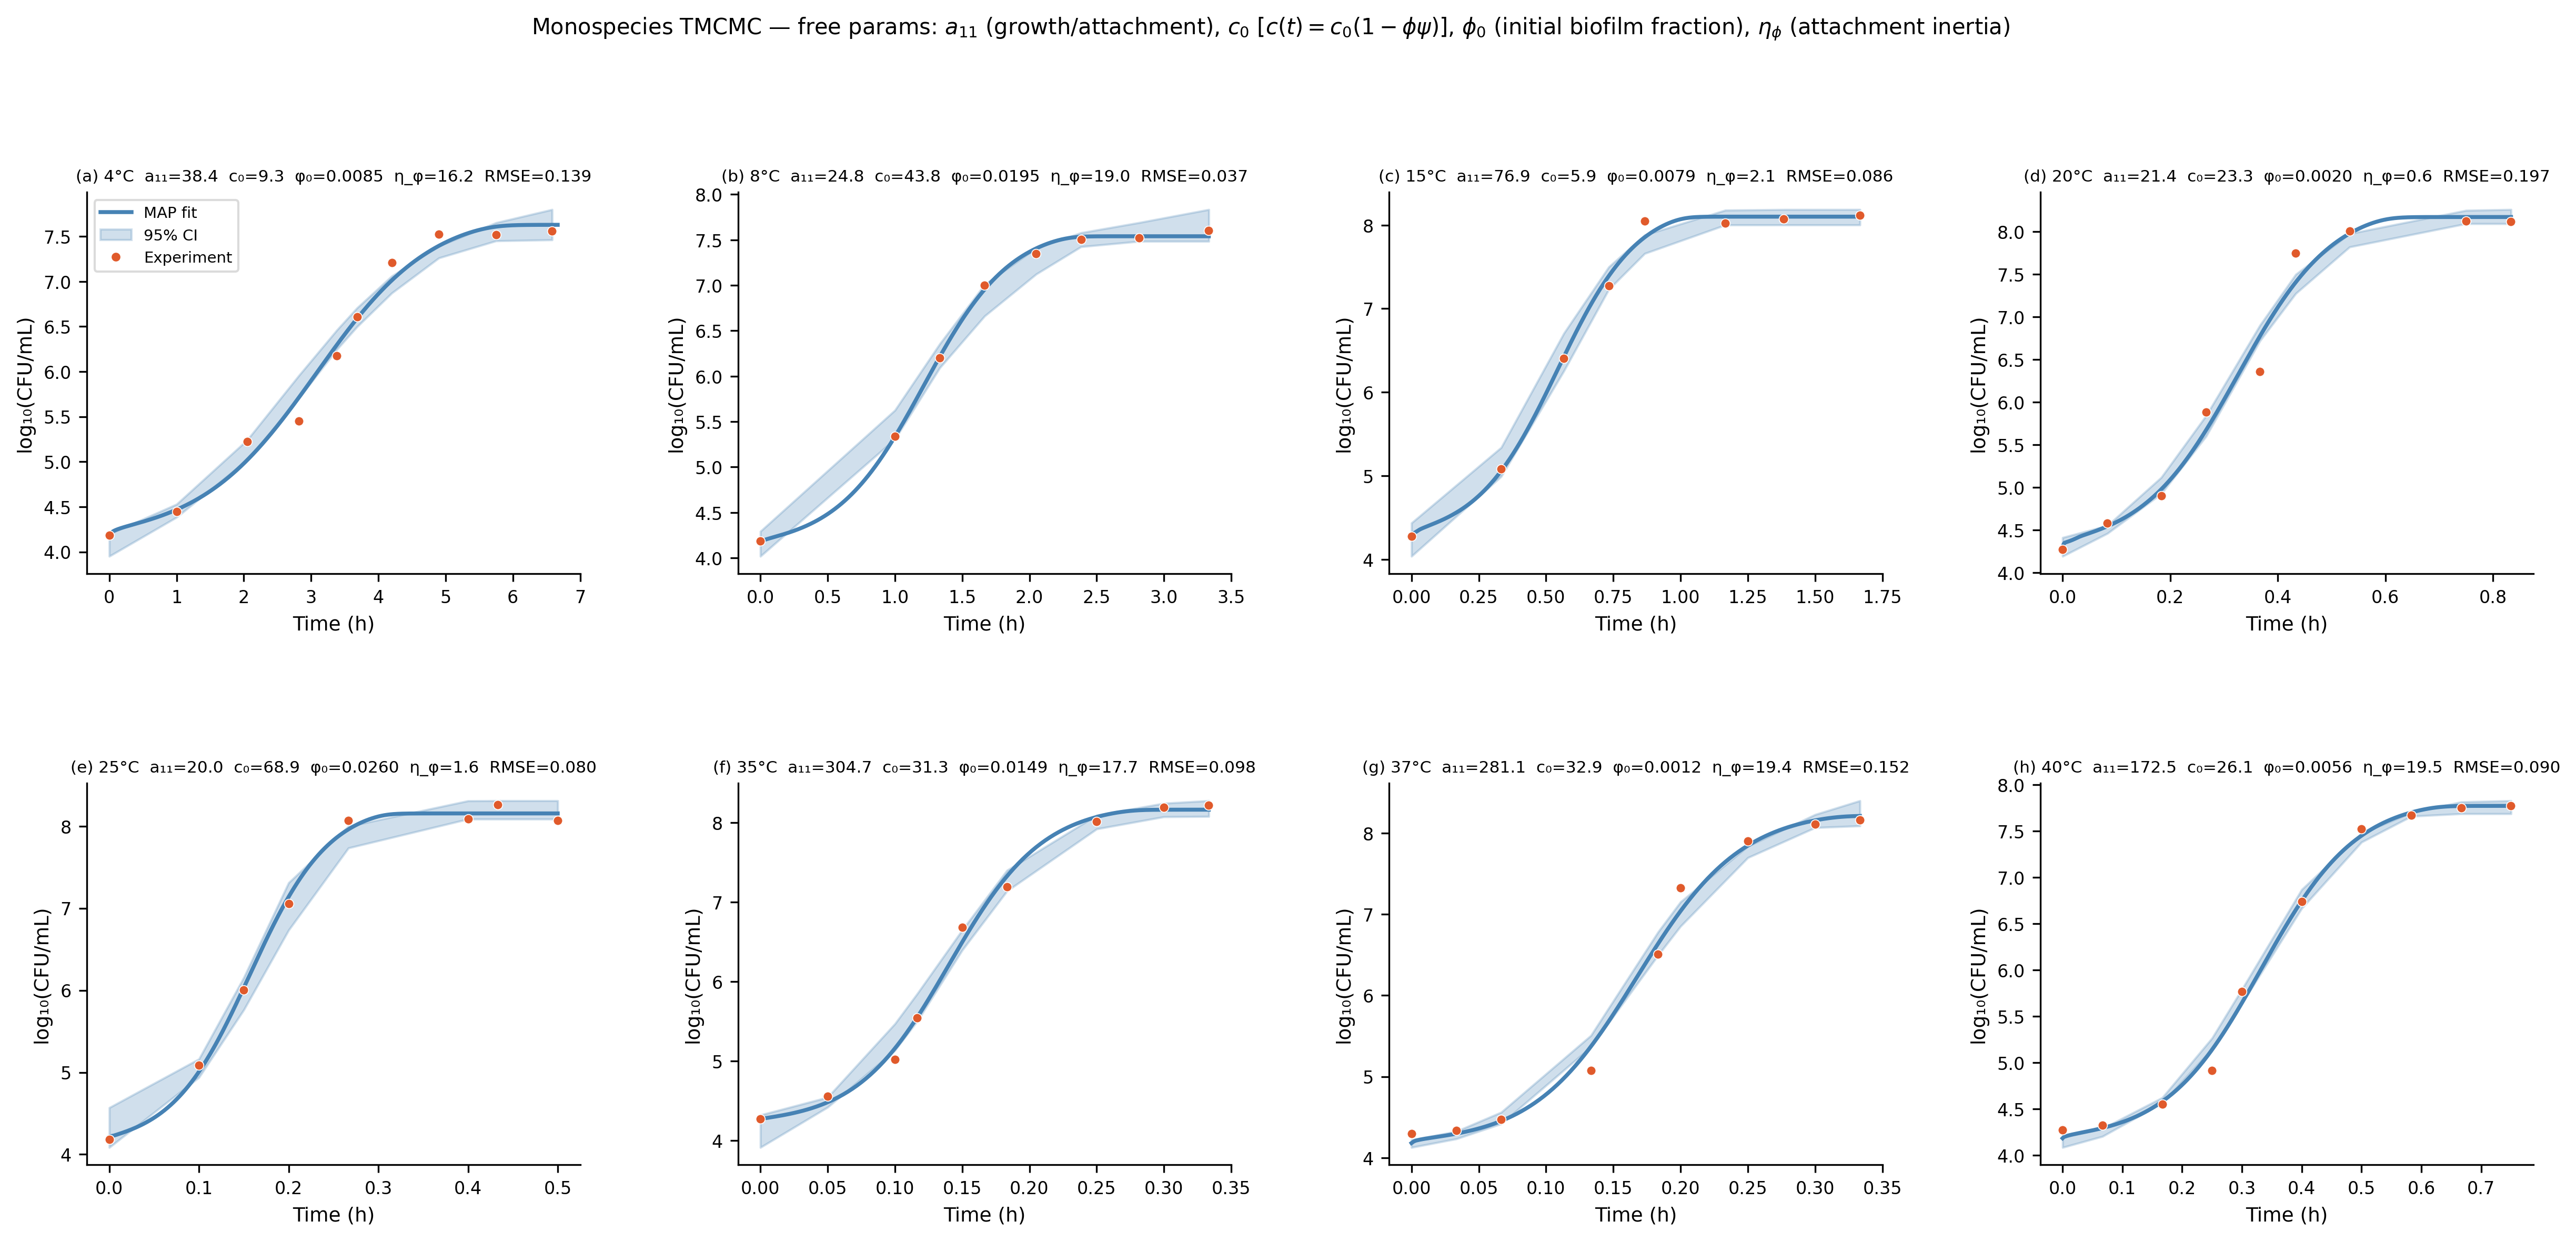
\includegraphics[width=\textwidth]{figures/monospecies_8panel_4param_fast.png}
\caption{M4 TMCMC ($\theta = a_{11}, c_{\mathrm{scale}}, \phi_0, \eta_\phi$; MAP + 95\% posterior predictive CI)
         for all eight temperatures. Blue: MAP trajectory; shaded band: 95\% CI; orange: experimental means.}
\label{fig:4d_8panel}
\end{figure}

% ─────────────────────────────────────────────────────────────────────────────
\section{Dynamic Temperature (Dy) Validation}
% ─────────────────────────────────────────────────────────────────────────────
\subsection{Experimental Setup}
The Dy experiment exposes the biofilm to a time-varying temperature profile
$T(t)$ spanning $\approx{-20}$\,°C to $40$\,°C over 150\,min \cite{liu2019}.
$N=24$ observations are available. The static $a_{11}$ knots (estimated from
$c_{\mathrm{scale}}=10$ runs) serve as the baseline for transfer models.

\subsection{Model Descriptions}
Three transfer strategies were compared:

\paragraph{1-var (1 param)}
\[
  a_{11}(t) = k\cdot \tilde{a}_{11}^{\mathrm{stat}}(T(t)), \quad \theta=(k).
\]
A single scalar $k$ scales the static knots interpolated at the current temperature.

\paragraph{Multi-knot (8 params)}
\[
  a_{11}(t) = \mathrm{interp}\!\bigl(k_i\cdot\tilde{a}_{11,i}^{\mathrm{stat}},\;T(t)\bigr),
  \quad \theta=(k_1,\ldots,k_8),
\]
allowing independent scaling at each of the eight reference temperatures.

\paragraph{Ratkowsky (5 params)}
\begin{align}
  \sqrt{a_{11,\mathrm{base}}(T)} &= b\,(T-T_{\min})\bigl[1-\exp(c(T-T_{\max}))\bigr],\\
  a_{11}(t) &= a_{11,\mathrm{base}}(T(t))\cdot\frac{1}{1+k_{\mathrm{lag}}|dT/dt|},
  \quad \theta=(b,T_{\min},T_{\max},c,k_{\mathrm{lag}}).
\end{align}

\subsection{Results}
TMCMC was run with $N_p=4000$ RW particles (Stuttgart GPU servers).

\begin{table}[h]
\centering
\caption{Dy model comparison ($N=24$ observations, $\sigma_{\mathrm{obs}}=0.1$\,fixed).}
\begin{tabular}{lcccccc}
\toprule
Model & Params & RMSE & $\log L$ & AIC & BIC \\
\midrule
1-var       & 1 & 0.1576 & 25.45 & $-$48.9 & $-$47.7 \\
Multi-knot  & 8 & 0.1332 & 48.86 & $-$81.7 & $-$72.3 \\
\textbf{Ratkowsky}   & \textbf{5} & \textbf{0.0904} & \textbf{45.46} & $\mathbf{-80.9}$ & $\mathbf{-75.0}$ \\
\bottomrule
\end{tabular}
\label{tab:dy_comparison}
\end{table}

Ratkowsky MAP: $b=0.327$, $T_{\min}=-0.81$\,°C, $T_{\max}=47.49$\,°C,
$c=1.258$, $k_{\mathrm{lag}}=2.2\times10^{-4}$.

Conclusions:
\begin{itemize}
  \item Ratkowsky achieves the lowest RMSE and best BIC among the three models.
  \item The near-zero $k_{\mathrm{lag}}$ MAP suggests the symmetric lag penalty is
        not yet capturing the true biological hysteresis.
  \item Multi-knot achieves higher $\log L$ but is penalised by AIC/BIC for the
        additional 7 parameters.
\end{itemize}

\begin{figure}[h]
\centering
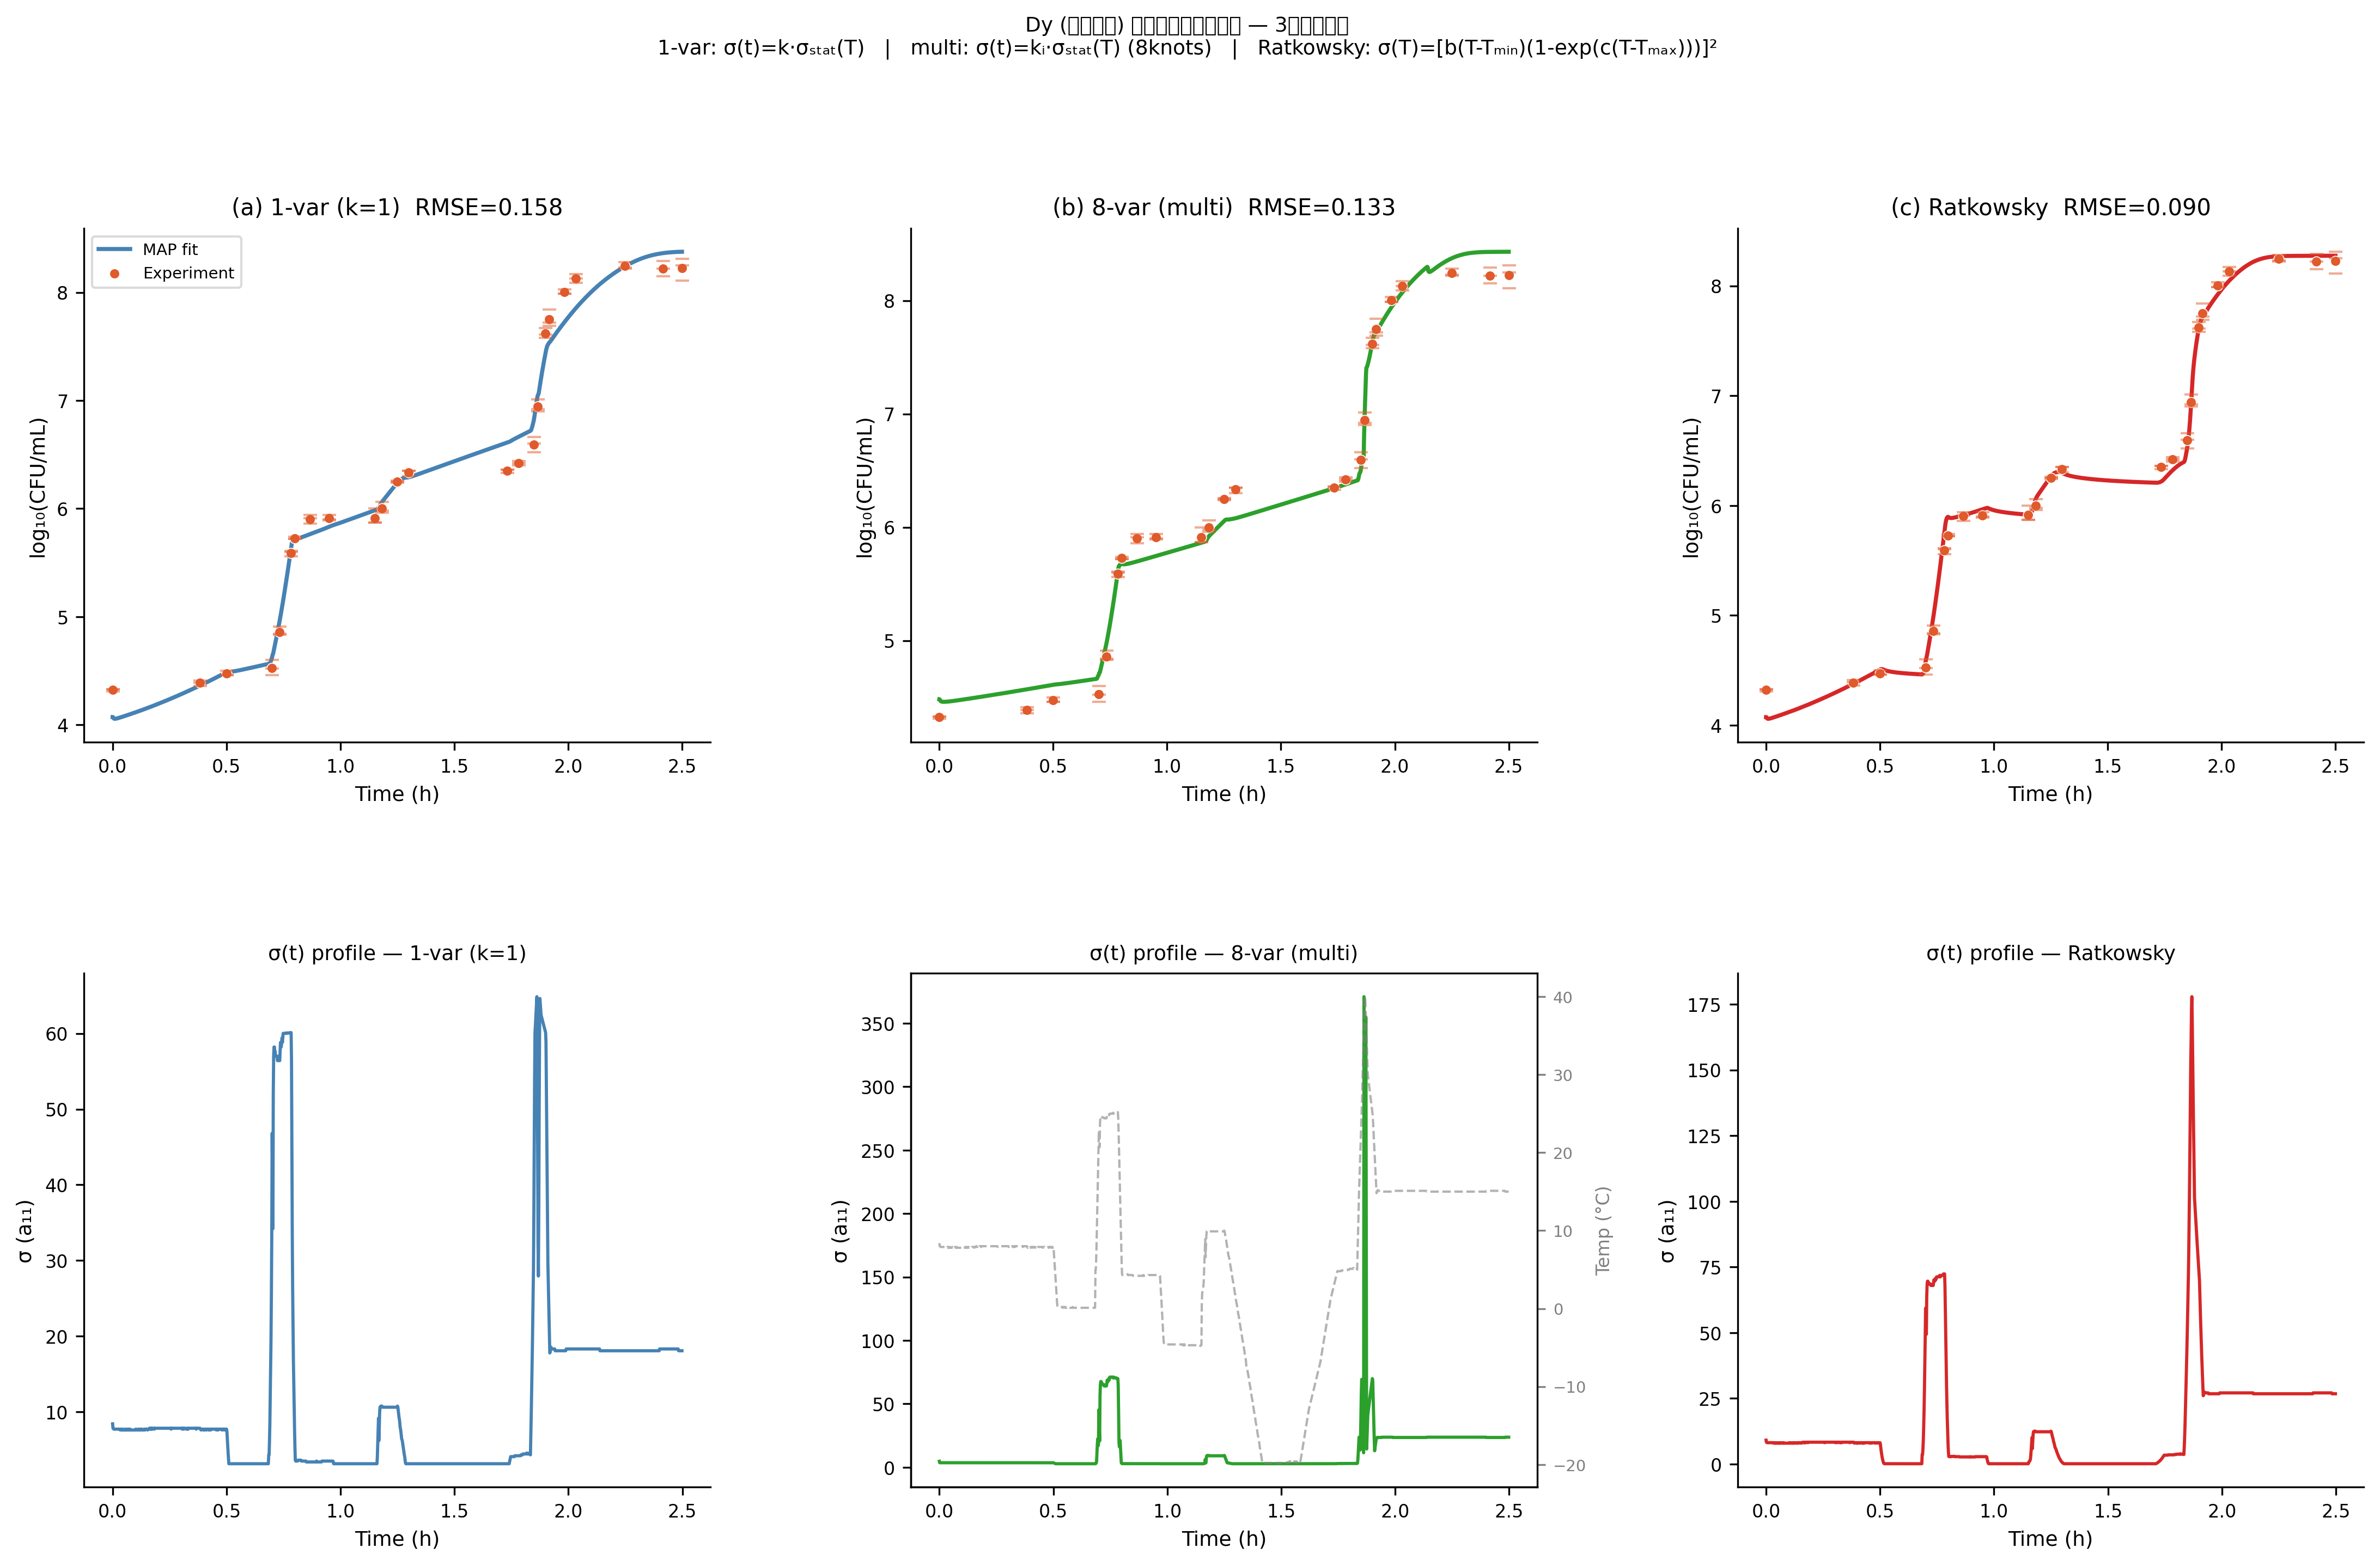
\includegraphics[width=\textwidth]{figures/dy_3model_comparison.png}
\caption{Dy data: MAP fit (top) and $a_{11}(t)$ profile (bottom) for the three
         transfer models. Temperature overlay (dashed grey) on $\sigma(t)$ panels.}
\label{fig:dy_3model}
\end{figure}

% ─────────────────────────────────────────────────────────────────────────────
\section{Enhanced $a_{11}(T,t)$ Models}
% ─────────────────────────────────────────────────────────────────────────────
\subsection{Motivation}
The near-zero $k_{\mathrm{lag}}$ in the Ratkowsky MAP and the experiment reaching
sub-zero temperatures ($T\approx{-20}$\,°C) motivate three physical extensions:

\begin{enumerate}
  \item \textbf{Thermal memory}: Cells respond to a time-averaged temperature,
        not the instantaneous $T(t)$.
  \item \textbf{Asymmetric lag}: Rapid cooling causes more damage than rapid
        heating (cold-shock vs.\ heat-shock asymmetry).
  \item \textbf{Cardinal Temperature Model (CTM)}: Physically motivated
        alternative to Ratkowsky, with explicit $T_{\mathrm{opt}}$.
\end{enumerate}

\subsection{Model Definitions}

\paragraph{CTM / Rosso 1995 (5 params) \cite{rosso1995}}
\begin{equation}
  a_{11}^{\mathrm{CTM}}(T)=\mu_{\mathrm{opt}}\cdot
  \frac{(T-T_{\max})(T-T_{\min})^2}
       {(T_{\mathrm{opt}}-T_{\min})
        \bigl[(T_{\mathrm{opt}}-T_{\min})(T-T_{\mathrm{opt}})
              -(T_{\mathrm{opt}}-T_{\max})(T_{\mathrm{opt}}+T_{\min}-2T)\bigr]},
  \quad \theta=(\mu_{\mathrm{opt}},T_{\min},T_{\mathrm{opt}},T_{\max},k_{\mathrm{lag}}).
\end{equation}

\paragraph{Thermal memory (Rat+$\tau$, 6 params)}
\begin{equation}
  T_{\mathrm{eff}}(t)=\int_{-\infty}^{t}T(s)\,\frac{e^{-(t-s)/\tau}}{\tau}\,ds
  \;\approx\; \alpha\,T_{\mathrm{eff}}(t{-}\Delta t)+(1-\alpha)\,T(t),
  \quad \alpha=e^{-\Delta t/\tau},
\end{equation}
then $a_{11}(t)=a_{11}^{\mathrm{Rat}}(T_{\mathrm{eff}}(t))$.
Extra parameter: $\log\tau\in[-3,4]$ (i.e.\ $\tau\in[0.05,\,54]$\,min).

\paragraph{Asymmetric lag (Rat+asym, 6 params)}
\begin{equation}
  a_{11}(t)=a_{11,\mathrm{base}}(T(t))\cdot
  \frac{1}{1+k(t)\,|dT/dt|},
  \quad k(t)=\begin{cases}k_{\mathrm{cool}}&\text{if }dT/dt<0\\k_{\mathrm{heat}}&\text{otherwise.}\end{cases}
\end{equation}

\paragraph{Full composite (Rat+$\tau$+asym, 7 params)}
Combines thermal memory on $T_{\mathrm{eff}}$ with asymmetric lag:
$\theta=(b,T_{\min},T_{\max},c,k_{\mathrm{cool}},k_{\mathrm{heat}},\log\tau)$.

\paragraph{CTM+$\tau$ (6 params)}
CTM evaluated at $T_{\mathrm{eff}}$ with symmetric lag.

\subsection{Estimation Strategy}
All six models are estimated via TMCMC with RW mutation and GPU \texttt{vmap},
$N_p=2000$ particles, on vancouver01 (4$\times$RTX~4090).
Script: \texttt{estimate\_monospecies\_tmcmc\_dy\_enhanced.py}.

\begin{table}[h]
\centering
\caption{Enhanced model comparison (TMCMC, $N_p=2000$ RW, vancouver01 RTX~4090, $N=24$ obs).}
\begin{tabular}{llccccl}
\toprule
Key & Label & $k$ & $\log L$ & AIC & BIC & Note \\
\midrule
\texttt{rat5}     & Ratkowsky          & 5 & \textbf{45.46} & \textbf{$-$80.9} & \textbf{$-$75.0} & \textbf{winner} \\
\texttt{rat\_mem} & Rat + $\tau$       & 6 & 45.60 & $-$79.2 & $-$72.1 & $\tau\approx0.06$\,min $\approx0$ \\
\texttt{ctm5}     & CTM-Rosso          & 5 & 44.10 & $-$78.2 & $-$72.3 & slightly inferior \\
\texttt{rat\_full}& Rat + $\tau$ + asym& 7 & 30.26 & $-$46.5 & $-$38.3 & overfitting \\
\texttt{rat\_asym}& Rat + asym lag     & 6 & 25.19 & $-$38.4 & $-$31.3 & overfitting ($k_{\rm heat}=8$) \\
\bottomrule
\end{tabular}
\label{tab:enhanced_models}
\end{table}

\subsection{Interpretation}
\begin{itemize}
  \item \textbf{Thermal memory} ($\tau$): MAP gives $\tau=\exp(-2.80)\approx0.06$\,min, essentially
        zero. The Dy temperature profile changes slowly enough that
        instantaneous $T(t)$ already captures the relevant dynamics.
  \item \textbf{Asymmetric lag}: Both \texttt{rat\_asym} and \texttt{rat\_full} degrade sharply.
        The heating lag $k_{\rm heat}=8$ absorbs variance that the base model handles via
        $T_{\min}/T_{\max}$ — an artefact of over-parameterisation on $N=24$ points.
  \item \textbf{CTM vs Ratkowsky}: CTM has a physically interpretable $T_{\rm opt}=38.1$\,°C
        consistent with \textit{Listeria} optima, but its slightly lower $\log L$ suggests the
        Ratkowsky formula fits the sub-zero decline better.
  \item \textbf{Conclusion}: The 5-parameter Ratkowsky model is confirmed as the best
        $a_{11}(T)$ model for the Dy validation.
\end{itemize}

\begin{figure}[h]
\centering
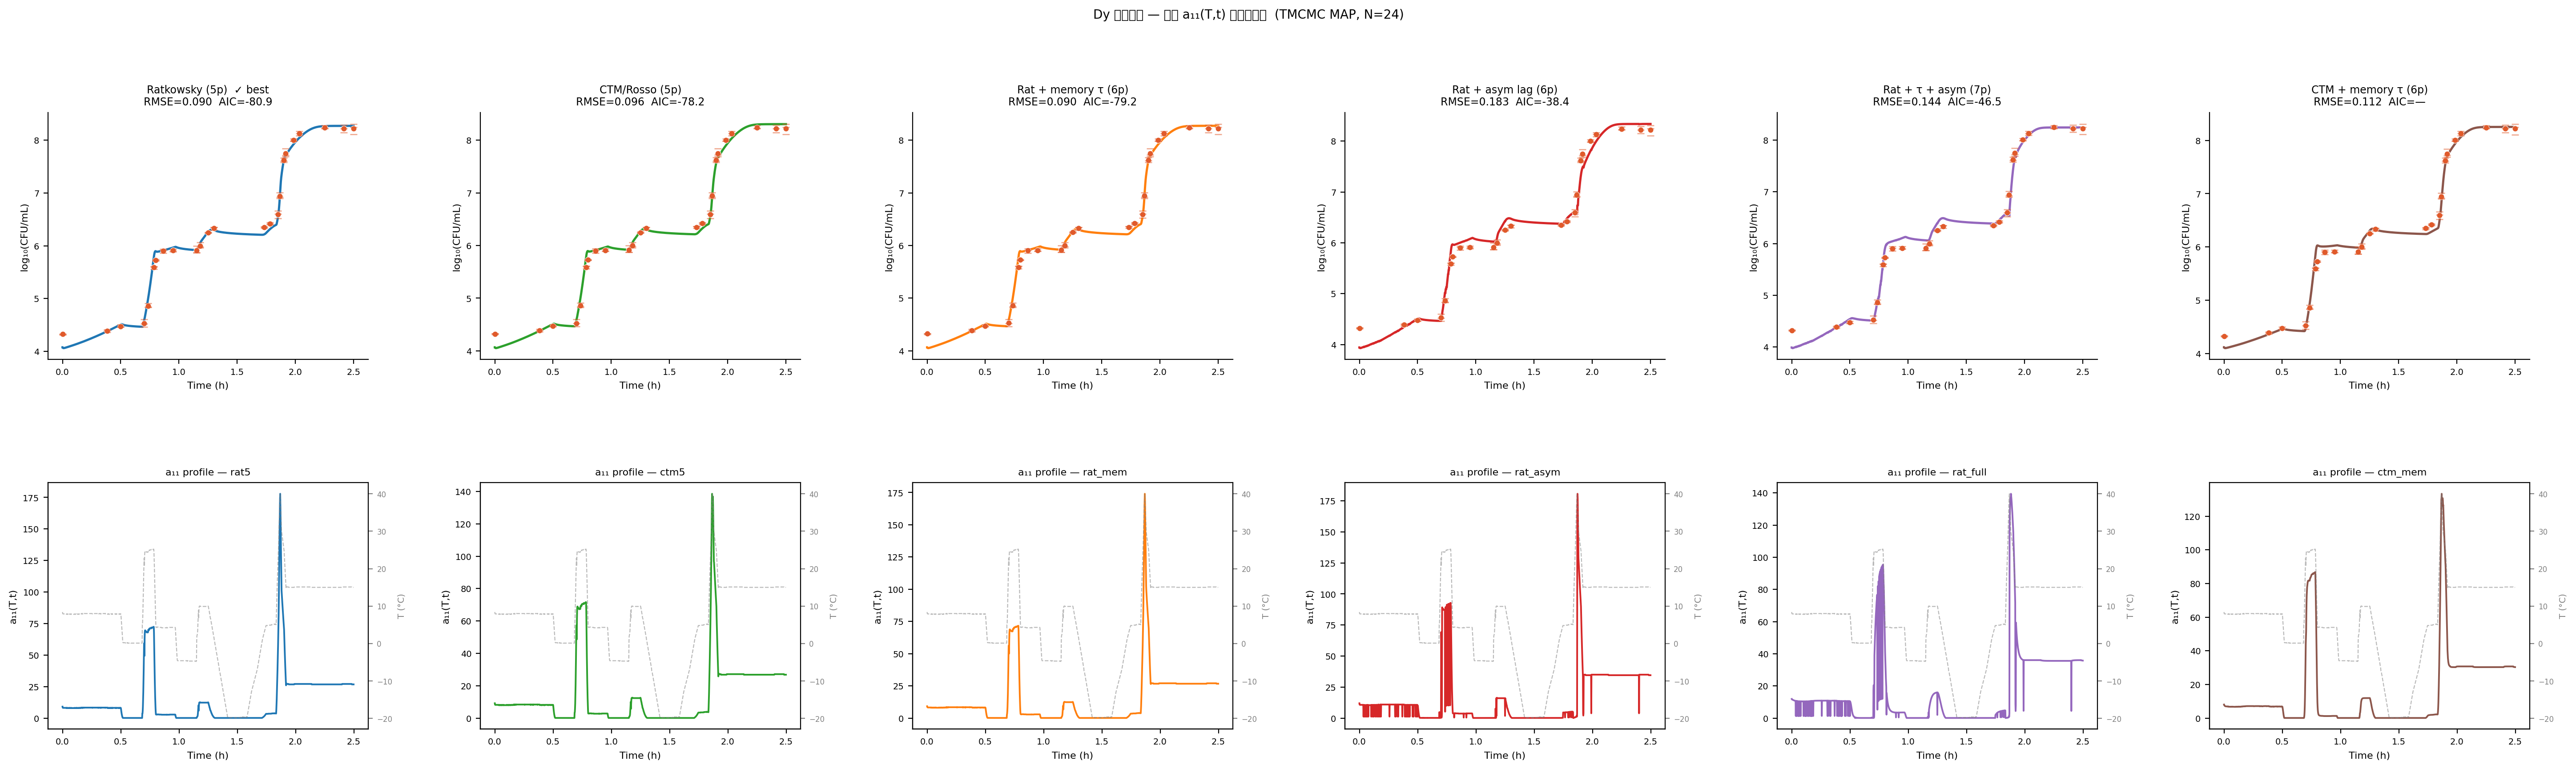
\includegraphics[width=\textwidth]{figures/dy_enhanced_model_comparison.png}
\caption{Enhanced $a_{11}(T,t)$ model comparison on Dy data. Top row: MAP fit vs.\ observed
         CFU (orange scatter); bottom row: $a_{11}(t)$ profile with temperature overlay (dashed
         grey). RMSE and AIC shown in each title. \texttt{rat\_asym} and \texttt{rat\_full} show
         clear over-fitting (flat $a_{11}$ during cooling phase).}
\label{fig:dy_enhanced}
\end{figure}

% ─────────────────────────────────────────────────────────────────────────────
\section{Discussion}
% ─────────────────────────────────────────────────────────────────────────────
\begin{itemize}
  \item The M4 static model consistently outperforms M1 and M3, confirming that
        both $c_{\mathrm{scale}}$ and $\eta_\phi$ are identifiable from the CFU
        time series.
  \item For the Dy validation, Ratkowsky outperforms both 1-var and multi-knot
        models in RMSE and BIC. Its $T_{\min}\approx -0.8$\,°C matches known
        growth limits for \textit{Listeria} \cite{liu2019}.
  \item The near-zero $k_{\mathrm{lag}}$ and the TMCMC results for extended models
        confirm that neither thermal memory nor asymmetric lag improves the fit
        on this dataset: the Dy temperature ramp is slow enough that
        instantaneous $T(t)$ already characterises growth adequately.
  \item GPU \texttt{vmap} TMCMC (vancouver01, RTX~4090) reduced wall-time for
        2000-particle runs to minutes, enabling systematic comparison of all
        six model variants.
\end{itemize}

% ─────────────────────────────────────────────────────────────────────────────
\section{Reproducibility}
% ─────────────────────────────────────────────────────────────────────────────
\begin{verbatim}
# Static M4 estimation (all 8 temperatures)
python3 estimate_monospecies_tmcmc_4param.py \
    --outdir _tmcmc_results_4param --n_particles 4000

# Dy baseline models
python3 estimate_monospecies_tmcmc_dy_ratkowsky.py \
    --outdir _tmcmc_results_dy_ratkowsky_rw4000p --n_particles 4000

# Dy enhanced models (vancouver01, GPU)
python3 estimate_monospecies_tmcmc_dy_enhanced.py \
    --model rat_full --n_particles 2000 \
    --outdir _tmcmc_results_dy_rat_full

# Visualization
python3 postprocess_dy.py
python3 postprocess_dy_enhanced.py
\end{verbatim}

\begin{thebibliography}{9}
\bibitem{liu2019}
Liu, Y., Wang, X., Liu, B., and Dong, Q. (2019).
One-Step Analysis for \textit{Listeria monocytogenes} Growth in
Ready-to-Eat Braised Beef at Dynamic and Static Conditions.
\textit{Journal of Food Protection}, 82(11):1820--1827.
\href{https://doi.org/10.4315/0362-028X.JFP-18-574}{doi:10.4315/0362-028X.JFP-18-574}.

\bibitem{ratkowsky1982}
Ratkowsky, D. A., Olley, J., McMeekin, T. A., and Ball, A. (1982).
Relationship between temperature and growth rate of bacterial cultures.
\textit{Journal of Bacteriology}, 149(1):1--5.
\href{https://doi.org/10.1128/jb.149.1.1-5.1982}{doi:10.1128/jb.149.1.1-5.1982}.

\bibitem{rosso1995}
Rosso, L., Lobry, J. R., Bajard, S., and Flandrois, J. P. (1995).
Convenient model to describe the combined effects of temperature and
pH on microbial growth.
\textit{Applied and Environmental Microbiology}, 61(2):610--616.
\href{https://doi.org/10.1128/aem.61.2.610-616.1995}{doi:10.1128/aem.61.2.610-616.1995}.

\bibitem{ching2007}
Ching, J. and Chen, Y.-C. (2007).
Transitional Markov Chain Monte Carlo method for Bayesian model
updating, model class selection, and model averaging.
\textit{Journal of Engineering Mechanics}, 133(7):816--832.
\href{https://doi.org/10.1061/(ASCE)0733-9399(2007)133:7(816)}{doi}.
\end{thebibliography}

\end{document}
